\documentclass{article}
\usepackage{graphicx} % Required for inserting images
\usepackage{geometry}
\usepackage{circuitikz}
\usepackage{siunitx}
\usepackage{CJKutf8}
\usepackage{amsmath}
\usepackage{amssymb}
\usepackage{caption}
\usepackage{float}
\usepackage{subcaption}
\geometry{top=5mm, left=30mm, a4paper}

\title{Oscillators and Signal Generators Prelab}
\author{梁程捷 (B11901136), 吳奕娃 (B11901080)}
\date{}


\begin{document}
\begin{CJK*}{UTF8}{bkai}

\maketitle

\section{Wein-Bridge Oscillator}
Construct the circuit in Figure (a), and follow the steps below: \\
1. Adjust the variable resistor until the sinusoidal vibration with the minimum amplitude occurs in $V_o$. Record $V_o$, f and the resistance of the variable resistor.\\
2. Adjust the variable resistor until the sinusoidal vibration with the maximum amplitude occurs in $V_o$. Record $V_o$, f and the resistance of the variable resistor. \\
3. Remove 1N4001, 1 \unit{\kilo\ohm}  and 3 \unit{\kilo\ohm}, and adjust the variable resistor. Make a conclusion according to the experimental results. \\

\section{Generation of Triangular and Square Waveforms}
Construct the circuit in Figure (b), and follow the steps below: \\
1. Record the output waveforms of CH 1 and CH 2 in Y-t mode. \\
2. Record the output frequency of this circuit. \\
3. Make a conclusion according to the experimental results. \\

\begin{figure}[h]
    \begin{center}
        \begin{subfigure}[b]{0.38\textwidth}
            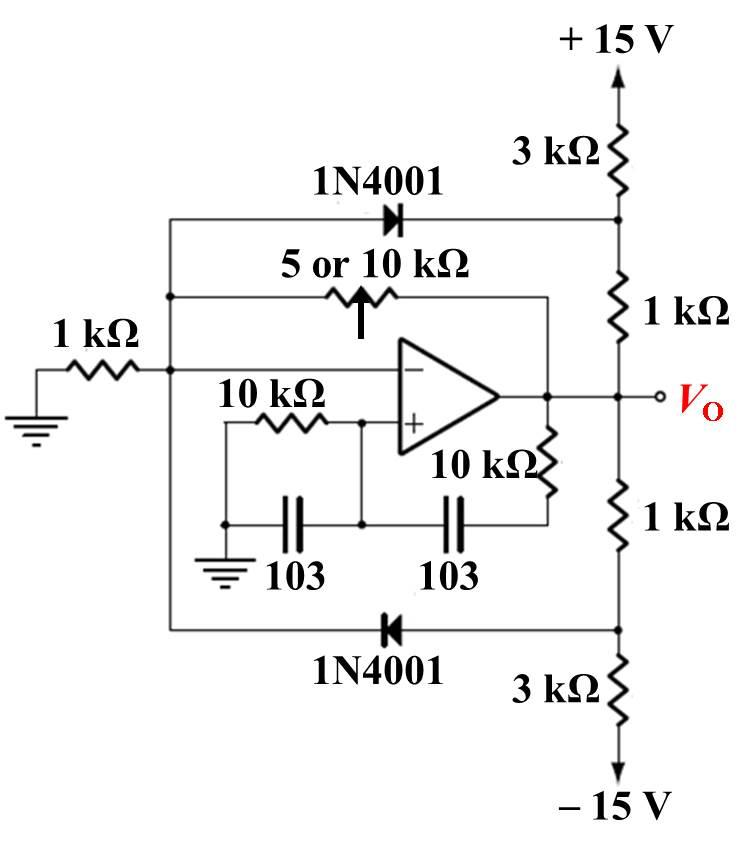
\includegraphics[width=\textwidth]{wein-bridge.png}
            \caption*{Figure (a): the Wein-Bridge oscillator circuit}
        \end{subfigure}
        ~
        \begin{subfigure}[b]{0.55\textwidth}
            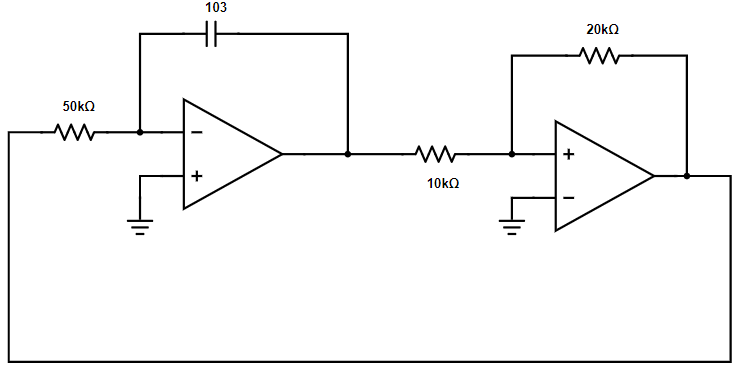
\includegraphics[width=\textwidth]{gen_tri_and_squ.png}
            \caption*{Figure (b): the circuit for generation of triangular and
square waveforms}
        \end{subfigure}
    \end{center}
\end{figure}
    
\end{CJK*}
\end{document}